\section*{Exercice 1?? -- SLCI Calculs}
% CCS PSI 2018

\setcounter{exo}{0}

Soient les modèles suivants. L'effort est donné par $f_c(t)=bK_f q(t)$. La quantité de matière enlevée est donnée par $q(t)=q_c(t)-z_2(t)+z_2(t-\tau)$ où $\tau est la durée nécessaire à la roue pour effectuer un tour complet.
D’un point de vue numérique, $K_f = \SI{1,5e9}{N.m^{-1}}$ et $\tau = \SI{1}{s}$. Le modèle de la chaîne d’asservissement est représenté par le schéma suivant.

 
\begin{center}
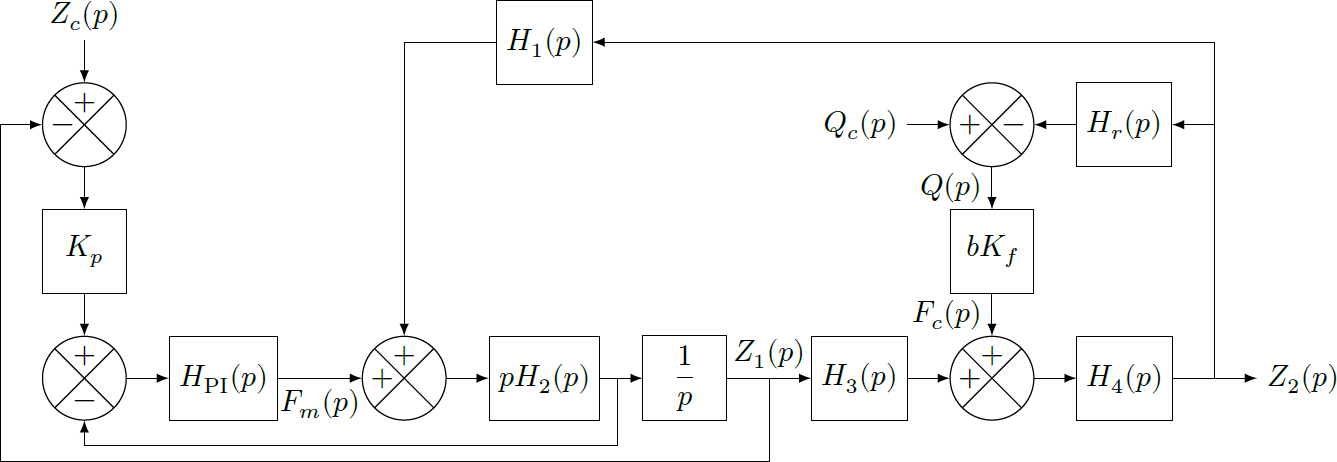
\includegraphics[width=1.0\linewidth]{049_01.png}
\end{center}


\subparagraph{}\textit{Déterminer $H_r(p)$ en fonction de $\tau$.}

\ifprof
\begin{corrige}
\end{corrige}
\else
\fi

En prenant $Z_c(p)=0$, le modèle précédent peut se mettre sous la forme du modèle équivalent suivant.

\begin{center}
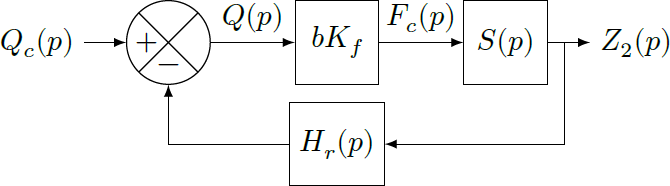
\includegraphics[width=1.0\linewidth]{049_02.png}
\end{center}

La figure suivante représente le diagramme de Bode de la fonction de transfert en boucle ouverte du système modélisé
figure précédemment, avec $b=\SI{5\times 10^{-2}}{\pi} \text{mm rad}^{-1}$. 


\subparagraph{}\textit{}
\ifprof
\begin{corrige}
\end{corrige}
\else
\fi